%!TEX TS-program = xelatex
\documentclass[12pt,a4paper, oneside]{extreport}

%%%%%%%%%% Математика %%%%%%%%%%
\usepackage{amsmath,amsfonts,amssymb,amsthm,mathtools}
% Показывать номера только у тех формул, на которые есть \eqref{} в тексте.
%\mathtoolsset{showonlyrefs=true}
%\usepackage{leqno} % Нумерация формул слева
%\usepackage{tipa} %Для формулки из логитов


\usepackage{hyphenat}


%%%%%%%%%% Шрифты %%%%%%%%
\usepackage[english, russian]{babel} % выбор языка для документа
\usepackage[utf8]{inputenc} % задание utf8 кодировки исходного tex файла
\usepackage[X2,T2A]{fontenc}        % кодировка

\usepackage{fontspec}         % пакет для подгрузки шрифтов
\setmainfont{Times New Roman}       % задаёт основной шрифт документа

\usepackage{unicode-math}      % пакет для установки математического шрифта
\setmathfont{Asana-Math.otf}    % шрифт для математики

% Конкретный символ из конкретного шрифта
% \setmathfont[range=\int]{Neo Euler}




%%%%%%%%%% Работа с картинками %%%%%%%%%
\usepackage{graphicx}                  % Для вставки рисунков
\usepackage{graphics}
\graphicspath{{images/}{pictures/}}    % можно указать папки с картинками
\usepackage{wrapfig}                   % Обтекание рисунков и таблиц текстом


%%%%%%%%%% Работа с таблицами %%%%%%%%%%
\usepackage{tabularx}            % новые типы колонок
\usepackage{tabulary}            % и ещё новые типы колонок
\usepackage{array,delarray}      % Дополнительная работа с таблицами
\usepackage{longtable}           % Длинные таблицы
\usepackage{multirow}            % Слияние строк в таблице
\usepackage{float}               % возможность позиционировать объекты в нужном месте

\usepackage{booktabs}            % таблицы как в книгах
% Заповеди из документации к booktabs:
% 1. Будь проще! Глазам должно быть комфортно
% 2. Не используйте вертикальные линни
% 3. Не используйте двойные линии. Как правило, достаточно трёх горизонтальных линий
% 4. Единицы измерения - в шапку таблицы
% 5. Не сокращайте .1 вместо 0.1
% 6. Повторяющееся значение повторяйте, а не говорите "то же"
% 7. Есть сомнения? Выравнивай по левому краю!

%  вычисляемые колонки по tabularx
\newcolumntype{C}{>{\centering\arraybackslash}X}
\newcolumntype{L}{>{\raggedright\arraybackslash}X}
\newcolumntype{Y}{>{\arraybackslash}X}
\newcolumntype{Z}{>{\centering\arraybackslash}X}


%%%%%%%%%% Графика и рисование %%%%%%%%%%
\usepackage{tikz, pgfplots}      % язык для рисования графики из latex'a

%%%%%%%%%% Гиперссылки %%%%%%%%%%
\usepackage{xcolor}              % разные цвета

\usepackage{hyperref}
\hypersetup{
	unicode=true,           % позволяет использовать юникодные символы
	colorlinks=true,       	% true - цветные ссылки, false - ссылки в рамках
	urlcolor =blue,         % цвет ссылки на url
	linkcolor=black,        % внутренние ссылки
	citecolor=black,        % на библиографию
	breaklinks              % если ссылка не умещается в одну строку, разбивать ли ее на две части?
}


%%%%%%%%%% Другие приятные пакеты %%%%%%%%%
\usepackage{multicol}       % несколько колонок
\usepackage{verbatim}       % для многострочных комментариев
\usepackage{cmap} % для кодировки шрифтов в pdf

\usepackage{enumitem} % дополнительные плюшки для списков
%  например \begin{enumerate}[resume] позволяет продолжить нумерацию в новом списке

\usepackage{todonotes} % для вставки в документ заметок о том, что  осталось сделать
% \todo{Здесь надо коэффициенты исправить}
% \missingfigure{Здесь будет Последний день Помпеи}
% \listoftodos --- печатает все поставленные \todo'шки



%%%%%%%%%%%%%% ГОСТОВСКИЕ ПРИБАМБАСЫ %%%%%%%%%%%%%%%

%%% размер листа бумаги
\usepackage[paper=a4paper,top=15mm, bottom=15mm,left=35mm,right=10mm,includehead]{geometry}


\usepackage{setspace}
\setstretch{1.33}     % Межстрочный интервал
\setlength{\parindent}{1.5em} % Красная строка.


%\flushbottom       % Эта команда заставляет LaTeX чуть растягивать строки, чтобы получить идеально прямоугольную страницу
\righthyphenmin=2  % Разрешение переноса двух и более символов
\widowpenalty=10000  % Наказание за вдовствующую строку (одна строка абзаца на этой странице, остальное --- на следующей)
%\clubpenalty=10000  % Наказание за сиротствующую строку (омерзительно висящая одинокая строка в начале страницы)
\tolerance=1000     % Ещё какое-то наказание.


% Нумерация страниц сверху по центру
\usepackage{fancyhdr}
\pagestyle{fancy}
\fancyhead{ } % clear all fields
\fancyfoot{ } % clear all fields
\fancyhead[C]{\thepage}
% Чтобы не прорисовывалась черта!
\renewcommand{\headrulewidth}{0pt}


% Нумерация страниц с надписью "Глава"
\usepackage{etoolbox}
\patchcmd{\chapter}{\thispagestyle{plain}}{\thispagestyle{fancy}}{}{}


%%% Заголовки
\usepackage[indentfirst]{titlesec}{\raggedleft}
% Заголовки по левому краю
% опция identfirst устанавливает отступ в первом абзаце



% В Linux этот пакет сделан косячно. Исправляет это следующий непонятный кусок кода.
\makeatletter
\patchcmd{\ttlh@hang}{\parindent\z@}{\parindent\z@\leavevmode}{}{}
\patchcmd{\ttlh@hang}{\noindent}{}{}{}
\makeatother


% Редактирования Глав и названий
\titleformat{\chapter}
{\normalfont\large\bfseries}
{\thechapter }{0.5 em}{}

% Редактирование ненумеруемых глав chapter* (Введение и тп)
\titleformat{name=\chapter,numberless}
{\centering\normalfont\bfseries\large}{}{0.25em}{\normalfont}

% Убирает чеканутые отступы вверху страницы
\titlespacing{\chapter}{0pt}{-\baselineskip}{\baselineskip}

% Более низкие уровни
\titleformat{\section}{\bfseries}{\thesection}{0.5 em}{}
\titleformat{\subsection}{\bfseries}{\thesubsection}{0.5 em}{}

\titlespacing*{\section}{0 pt}{\baselineskip}{\baselineskip}
\titlespacing*{\subsection}{0 pt}{\baselineskip}{\baselineskip}


% Содержание. Команды ниже изменяют отступы и рисуют точечки!
\usepackage{titletoc}

\titlecontents{chapter}
[1em] %
{\normalsize}
{\contentslabel{1 em}}
{\hspace{-1 em}}
{\normalsize\titlerule*[10pt]{.}\contentspage}

\titlecontents{section}
[3 em] %
{\normalsize}
{\contentslabel{1.75 em}}
{\hspace{-1.75 em}}
{\normalsize\titlerule*[10pt]{.}\contentspage}

\titlecontents{subsection}
[6 em] %
{\normalsize}
{\contentslabel{3 em}}
{\hspace{-3 em}}
{\normalsize\titlerule*[10pt]{.}\contentspage}


% Правильные подписи под таблицей и рисунком
% Документация к пакету на русском языке!
\usepackage[tableposition=top, singlelinecheck=false]{caption}
\usepackage{subcaption}


\DeclareCaptionStyle{base}%
[justification=centering,indention=0pt]{}
\DeclareCaptionLabelFormat{gostfigure}{Рисунок #2}
\DeclareCaptionLabelFormat{gosttable}{Таблица #2}

\DeclareCaptionLabelSeparator{gost}{~---~}
\captionsetup{labelsep=gost}

\DeclareCaptionStyle{fig01}%
[margin=5mm,justification=centering]%
{margin={3em,3em}}
\captionsetup*[figure]{style=fig01,labelsep=gost,labelformat=gostfigure,format=hang}

\DeclareCaptionStyle{tab01}%
[margin=5mm,justification=centering]%
{margin={3em,3em}}
\captionsetup*[table]{style=tab01,labelsep=gost,labelformat=gosttable,format=hang}


% межстрочный отступ в таблице
\renewcommand{\arraystretch}{1.2}



% многостраничные таблицы под РОССИЙСКИЙ СТАНДАРТ
% ВНИМАНИЕ! Обязательно за CAPTION !
\usepackage{fr-longtable}



%Более гибкие спсики
\usepackage{enumitem}
% сообщаем окружению о том, что существует такая штук как нумерация русскими буквами.
\makeatletter
\AddEnumerateCounter{\asbuk}{\russian@alph}{щ}
\makeatother


%%% ГОСТОВСКИЕ СПИСКИ

% Первый тип списков. Большая буква.
\newlist{Enumerate}{enumerate}{1}

\setlist[Enumerate,1]{labelsep=0.5em,leftmargin=1.25em,labelwidth=1.25em,
	parsep=0em,itemsep=0em,topsep=0ex, before={\parskip=-1em},label=\arabic{Enumeratei}.}


% Второй тип списков. Маленькая буква.
\setlist[enumerate]{label=\arabic{enumi}),parsep=0em,itemsep=0em,topsep=0.75ex, before={\parskip=-1em}}


% Третий тип списков. Два уровня.
\newlist{twoenumerate}{enumerate}{2}
\setlist[twoenumerate,1]{itemsep=0mm,parsep=0em,topsep=0.75ex,, before={\parskip=-1em},label=\asbuk{twoenumeratei})}
\setlist[twoenumerate,2]{leftmargin=1.3em,itemsep=0mm,parsep=0em,topsep=0ex, before={\parskip=-1em},label=\arabic{twoenumerateii})}


% Четвёртый тип списков. Список с тире.
\setlist[itemize]{label=--,parsep=0em,itemsep=0em,topsep=0ex, before={\parskip=-1em},after={\parskip=-1em}}


%%% WARNING WARNING WARNIN!
%%% Если в списке предложения, то должна по госту стоять точка после цифры => команда Enumerate! Если идет перечень маленьких фактов, не обособляемых предложений то после цифры идет скобка ")" => команда enumerate! Если перечень при этом ещё и двууровневый, то twoenumerate.




%%%%%%%%%% Список литературы %%%%%%%%%%

%\usepackage[%
%backend=biber, %подключение пакета biber (тоже нужен)
%bibstyle=gost-numeric, %подключение одного из четырех главных стилей biblatex-gost
%sorting=ntvy, %тип сортировки в библиографии
%]{biblatex}
\usepackage[backend=biber,style=gost-numeric, maxbibnames=9,maxcitenames=2,uniquelist=false, babel=other]{biblatex}

% Справка по 4 главным стилям для ленивых:
% gost-inline  ссылки внутри теста в круглых скобках
% gost-footnote подстрочные ссылки
% gost-numeric затекстовые ссылки
% gost-authoryear тоже затекстовые ссылки, но немного другие

% Подробнее смотри страницу 4 документации. Она на русском.

% Ещё немного настроек
\DeclareFieldFormat{postnote}{#1} %убирает с. и p.
\renewcommand*{\mkgostheading}[1]{#1} % только лишь убираем курсив с авторов


\addbibresource{diplomabib.bib} % сюда нужно вписать свой bib-файлик.

% Этот кусок кода выносит русские источники на первое место. Костыль описали авторы пакета в руководстве к нему. Подробнее смотри:
% https://github.com/odomanov/biblatex-gost/wiki/Как-сделать%2C-чтобы-русскоязычные-источники-предшествовали-остальным
\DeclareSourcemap{
	\maps[datatype=bibtex]{
		\map{
			\step[fieldsource=langid, match=russian, final]
			\step[fieldset=presort, fieldvalue={a}]
		}
		\map{
			\step[fieldsource=langid, notmatch=russian, final]
			\step[fieldset=presort, fieldvalue={z}]
		}
	}
}

\DefineBibliographyStrings{english}{%
	pages = {P\adddot},
	number = {№},
}


\begin{document} % Начала документа

\thispagestyle{empty} % Чтобы избежать нумерации титульника

% Если для какой-то страницы хочется сделать своё уникальное оформление, как например для титульника или списка литературы, то можно использовать окружение \begingroup ... \endgroup. 
\begingroup
\setstretch{1}   % Убираем полторашные интервалы на титульнике
\begin{center}
\small \bfseries Федеральное государственное бюджетное образовательное учреждение высшего образования

<<РОССИЙСКАЯ АКАДЕМИЯ НАРОДНОГО ХОЗЯЙСТВА и\\ ГОСУДАРСТВЕННОЙ СЛУЖБЫ \\
при Президенте Российской Федерации>>

\vspace{2ex}

\bfseries
ИНСТИТУТ ЭКОНОМИКИ, МАТЕМАТИКИ И ИНФОРМАЦИОННЫХ 

ТЕХНОЛОГИЙ
 
 ЭКОНОМИЧЕСКИЙ ФАКУЛЬТЕТ 
 
НАПРАВЛЕНИЕ 38.03.01 ЭКОНОМИКА

\end{center}

\vfill


\noindent  Группа ЭО-15-01
\hfill
\parbox[t]{20em}{\centering
Кафедра микроэкономики

\mbox{ }

\textbf{Допустить к защите}

заведующий кафедрой микроэкономики

\mbox{ }

\rule{8em}{0.5pt} М.И. Левин

\mbox{ }

<<\rule{2em}{0.5pt}>> \rule{5em}{0.5pt} 201\rule{1em}{0.5pt} г. }

\mbox{ }

\mbox{ }

\begin{center}\bfseries
ВЫПУСКНАЯ КВАЛИФИКАЦИОННАЯ РАБОТА

\mbox{ }

\large
ПРОГНОЗИРОВАНИЕ   \\
ИЕРАРХИЧЕСКИХ ВРЕМЕННЫХ РЯДОВ
\end{center}

\vfill

\noindent\normalsize
студент-бакалавр

\noindent
Касьянова Ксения Алексеевна
\hfill /\rule{6em}{0.5pt}/\rule{6em}{0.5pt}/

\hfill\makebox[13em]{\hfill\footnotesize (подпись) \hfill\hfill (дата) \hfill}

\noindent
научный руководитель выпускной \\
квалификационной работы

\noindent
ст. преп. Демешев Борис Борисович
\hfill /\rule{6em}{0.5pt}/\rule{6em}{0.5pt}/

\hfill\makebox[13em]{\hfill\footnotesize (подпись) \hfill\hfill (дата) \hfill}

%\noindent
%консультант
%
%\noindent
%д.э.н., профессор Петров Петр Петрович
%\hfill /\rule{6em}{0.5pt}/\rule{6em}{0.5pt}/
%
%\hfill\makebox[13em]{\hfill\footnotesize (подпись) \hfill\hfill (дата) \hfill}

\vfill

\begin{center}
\normalsize \bfseries МОСКВА \\ 2019 г.
\end{center}
\endgroup



%%%%%%%%%%%%%%%%%%% ОГЛАВЛЕНИЕ %%%%%%%%%%%%%%%%%%%%%%%%%%%%%%%%%%%%%%

\tableofcontents  % Команда, которая создаёт оглавление


%%%%%%% ВВЕДЕНИЕ %%%%%%

\chapter*{Введение}
%Включение введения в соодержание
\addcontentsline{toc}{chapter}{Введение}


В анализе данных часто встречаются данные со сложной многоуровневой структурой, точный прогноз которых является одним из ключевых факторов принятия эффективных решений. В связи с этим необходимо использовать уже известные подходы, позволяющие учитывать взаимозависимости прогнозируемых временных рядов, и разрабатывать новые.  


С    развитием различных социально-экономических процессов, укрепляется и взаимосвязь между ними. Анализ данных с иерархической структурой требуется в микроэкономике (например, при анализе спроса на различные виды товаров в разных городах), макроэкономике (показатели выпуска по регионам по разным отраслям), страховании (анализ рисков попасть аварию, в зависимости от привычек и местонахождения человека),  демографии (смертность по регионам и причинам смерти) и т.д.  Помимо этого существует и межвременная агрегация временных рядов, часто применяющаяся при прогнозировании.  

В данной работе исследуются методы прогнозирования иерархических временных рядов, учитывающие зависимость между уровнями агрегирования и внутри одного уровня. Теоретической основой исследования послужили работы ученых в области анализа данных, прогнозирования и моделирования.



Цель работы: сравнение моделей, учитывающих иерархическую структуру данных, выявление факторов, позволяющих улучшить прогнозы агрегированного временного ряда.

%используя модели, учитывающие иерархическую структуру данных, улучшить прогнозы агрегированного временного ряда.

%использовать информацию на одном уровне агрегирования для улучшения прогнозов на другом уровне агрегирования. 

Достижение поставленной цели предполагает постановку и решение следующих задач:

\begin{itemize}
	\item сбор данных с трехуровневой иерархической структурой;
	\item выбор моделей для прогнозирования агрегированного ряда;
%	\item сравнение ARIMA моделей с использованием дополнительных регрессоров (ближайшего по метрике корреляции временного ряда третьего уровня, ряда второго уровня или прогноза ряда второго уровня) и без;    
	\item сравнение различных методов комбинирования прогнозов нижних рядов; 
	\item кластеризация временных рядов третьего уровня для получения комбинированных рядов второго уровня (суммирование всех рядов, попавших в один кластер), сравнение прогнозов по  "оригинальным" и "комбинированным" рядам второго уровня;
	\item прогнозирование рядов второго и третьего уровня по выбранным моделям, сравнение суммы и оптимальной комбинации этих прогнозов с прогнозом агрегированного временного ряда.
%	\item сравнение прогнозной силы моделей для агрегированного временного ряда, взвешенных прогнозов дизагрегированных рядов; % и иерархической байесовской модели.
%\item  Добавление в модель дамми структурного сдвига

\end{itemize}


%Актуальность
Методы, описанные в данной работе актуальны при необходимости прогнозирования, как агрегированного ряда, так и отдельных компонент, составляющих его, а также получения подтверждения правильности выбора модели для агрегированного ряда.
Для анализа были выбраны ряды с определенной структурой, а именно: 
структура трехуровневая и иерархическая, причем сам агрегированный ряд и ряды второго уровня можно получить при суммировании рядов третьего уровня. 
%В ходе исследования мы определим,  позволяет ли такое детальное дробление временного ряда на более мелкие добиться существенного улучшения прогнозов или можно, например, ограничиться двумя уровнями.


% теоретическую и практическую значимость работы (если работа претендует на значи-мые результаты в этих аспектах)

Практическая значимость работы заключается в том, что при анализе результатов применения изучаемых методов на трех наборах данных (с разной сезонностью, числом наблюдений и рядов на каждом уровне)   с использованием перекрестной проверки (кросс-валидации) можно протестировать методы на независимых данных, а следовательно получить более устойчивые  выводы. 



В результате проведенного анализа были получены три основных вывода: 

\begin{itemize}
	\item эффективность  моделей прогнозирования  агрегированных рядов с помощью моделей, учитывающих многоуровневую структуру данных,  сильно варьируется для разных наборов данных и зависит от структуры рядов-компонент   по отдельности;
\item комбинирование прогнозов с помощью OLS-корректировки  имеет смысл при небольшом числе наблюдений, недостаточном для проведения кросс-валидации, поскольку позволяет устранить сильное отклонение невзвешенной суммы прогнозов от прогноза агрегированного ряда по причине случайного накопления идиосинкразических ошибок;
\item     предварительная группировка рядов нижнего уровня перед прогнозированием практически во всех случаях приносит положительный результат, по сравнению с прогнозами полученными по трехуровневой модели. 
\end{itemize}



Данная работа состоит из введения, двух глав основной части, заключения и приложений. В первой главе рассматриваются основные модели прогнозирования иерархических временных рядов.  Во второй главе проводится  сравнение моделей применительно к собранным данным с требуемой структурой. 
В приложении \ref{app-a} содержатся графики, позволяющие визуализировать структуру данных. В приложении \ref{app-b} представлены таблицы, позволяющие сравнить качество прогнозов, полученное по  моделям, учитывающим многоуровневую  структуру данных с моделью, ее не учитывающей. 




% степень ее разработанности


%методологию и методы исследования;

%положения, выносимые на защиту;



\chapter{Модели прогнозирования временных рядов  с иерархической \\ структурой}



\section{Обзор литературы}

Одним из способов повышения точности прогнозов является агрегирование данных. Один из вариантов - агрегирование временных рядов до составления прогноза, другой - агрегирование самих прогнозов. 

С другой стороны информация полученная из аггрегированных рядов может иметь существенное влияние при прогнозировании рядов нижнего уровня, хотя ее использование может сопровождаться некоторыми сложностями. 

Для наиболее распространенных моделей прогнозированию существуют альтернативные подходы к анализу временных рядов с иерархической структурой, например, модель  векторной авторегрессии (VAR), в которой  временные ряды имеют общие параметры или модель байесовской векторной авторегрессии (BVAR), где коэффициенты  при различных регрессорах могут иметь общее априорное распределение.  В том числе применяются многомерные модели пространства состояний, векторное  экспоненциальное сглаживание, а также  байесовские подходы, например, их применение к пулу аналогичных временных рядов с помощью ... [Duncan et al. (1993, 2001)].
В таких моделях обычная оценка параметрами объединяется с оцененкой по сгруппированной модели. 

Эмпирические результаты показали, что с помощью перечисленных выше методов точность прогноза может быть улучшена, поскольку они используют ковариационную зависимость  между временными рядами. Однако использование их связано с выполнением большого числа предпосылок или введения соответствующих ограничений на модель.


Эти методы по крайней мере теоретически могут легко обогнать по качеству прогнозов такие простые подходы, как bottom-up (BU), top-down (TD).
Но помимо BU и TD подходов к получению прогнозов аггрегированных рядов, существуют более сложные методы получения  оптимальных комбинаций прогонозов, например, ...
Однако во многих теоретических и эмпирических работах было замечено, что зачастую более простые методы комбинирования прогнозов оказываются в разы эффективнее, сложных методов, использующих метррики, учитывающие особенности каждого из рядов. Так, например, в статье ... лучший прогноз давало простое взвешивание прогнозов. 



Одной из наиболее распространенных моделей прогнозирования взаимозависимых рядов является модель векторной авторегрессии (VAR), однако ее использование может сопровождаться некоторыми сложностями, например, при большое число лагов в модели приводит значительному росту числа оцениваемых коэффициентов.  

В качестве некой альтернативы этому методу можно предложить использование модели ARIMA с дополнительными регрессорами, полученными из прогнозируемого набора данных. 


\textbf{Forward	modelling:	}   with
noise	
properties	
we	
can	 predict	
the	Sampling	

Distribution
(the probability	
for	
a	
general	
set	
of	
data


In	
easy	
cases,	
the	
effect	
of	
the	
prior	
is	
simple. As	
experiment	
gathers	
more	
data,	
the	
likelihood	
tends	
to	
get	
narrower,	
and	
the	
influence	
of	
the	
prior	
diminishes.	


Rule	
of	
thumb:	
if	
changing	
your	
prior	
to	
another	
reasonable	
one	
changes	
the	
answers	
significantly,	
you	
need	
more	
data	

Bayesians claim that the parameters are random so that their credible interval is a valid probability argument, though it also depends on the  the prior, which is usually hard to obtain.

 When the likelihood and prior is complicated, the inference has to rely on the MCMC sampling, which can be really slow in most of the real-world cases.

 The biggest controversy about Bayesian inference is that you must quantify your prior knowledge about the question at hand. This makes it possible to actually influence your results, either accidentally or on purpose. 	


\textbf{Shrinkage} is implicit in Bayesian inference and penalized likelihood inference, and explicit in James–Stein-type inference. In contrast, simple types of maximum-likelihood and least-squares estimation procedures do not include shrinkage effects, although they can be used within shrinkage estimation schemes.


\textbf{Stein's  paradox}, in decision theory and estimation theory, is the phenomenon that when three or more parameters are estimated simultaneously, there exist combined estimators more accurate on average (that is, having lower expected mean squared error) than any method that handles the parameters separately. 

\textit{The best guess about the future is usually  obtained by computing the average of past events. Stein's paradox defines circumstances in which there are estimators better that the arithmetic average
}

Stein’s paradox  **modern generalization, the Bayesian hierarchical model**. 

Bayesian hierarchical model can improve overall estimation accuracy, thereby improving our confidence in the assessment results, especially for standard compliance assessment of waters with **small sample sizes.**


\section{Взвешенные прогнозы}




The assumption upon which many of these models are built on, is that by grouping series that behave in a similar way, the idiosyncratic errors within groups will tend to offset each other while the more relevant individual dynamics will be retained to be modelled.



Key idea: forecast reconciliation
\begin{itemize}
	\item Ignore structural constraints and forecast
	every series of interest independently.
	\item Adjust forecasts to impose constraints.
\end{itemize}

Existing methods:
\begin{itemize}
	\item  Bottom-up
	\item  Top-down
	\item  Middle-out
	
\end{itemize}

An “optimal combination” 
approach can be advanced by proposing two new estimators
based on WLS.

Both now implemented in the hts package

$ Y_t $ : observed aggregate of all
series at time $ t $.

$ Y_{ X , t} $ : observation on series X at
time t.




For the hierarchical structure we can write: 

\[\begin{bmatrix}
y_{t} \\
y_{A, t} \\
y_{B, t} \\
y_{AA, t} \\
y_{AB, t} \\
y_{AC, t} \\
y_{BA, t} \\
y_{BB, t}
\end{bmatrix}
=
\begin{bmatrix}
1 & 1 & 1 & 1 & 1 \\
1 & 1 & 1 & 0 & 0 \\
0 & 0 & 0 & 1 & 1 \\
1  & 0  & 0  & 0  & 0  \\
0  & 1  & 0  & 0  & 0  \\
0  & 0  & 1  & 0  & 0  \\
0  & 0  & 0  & 1  & 0  \\
0  & 0  & 0  & 0  & 1
\end{bmatrix}
\begin{bmatrix}
y_{AA, t} \\
y_{AB, t} \\
y_{AC, t} \\
y_{BA, t} \\
y_{BB, t}
\end{bmatrix}\]


or in more compact notation,  where  $y_t$   is an $n$-dimensional vector of all the observations in the hierarchy at time $t$, $S$  is the summing matrix.

$$y_t  = S b_t$$


$ b_t $ : $m$-dimensional vector of all series at
bottom level in time t.





\[ \hat{Y}_n ( h ) = S \beta_n ( h ) + e_h  \]

$ \hat{Y}_n ( h ) $ - a vector of initial $ h $-step forecasts,
made at time $ n $, stacked in same order as $ Y_t  $.

$ \beta_n ( h )   = E [ B _{n + h} | Y_1 , \dots , Y_n ]  $

$ e_h  $  has zero mean and covariance $ \Sigma_h  $.

\[ \tilde{Y}_n ( h )
= S \hat{\beta}_n ( h ) = S P  \hat{Y}_n ( h ) =  S ( S' \Sigma^{+}_h S )^{-1}  S'  \Sigma^{+}_h  \hat{Y}_n ( h )
\]

$ \tilde{Y}_n ( h ) $   - revised forecasts, 
$ \hat{Y}_n ( h ) $ - initial forecasts

$ \Sigma^{+}_h $ - generalized inverse of $ \Sigma_h $.

Optimal $ P = ( S' \Sigma^{+}_h S )^{-1}  S'  \Sigma^{+}_h  $

Problem: $ \Sigma_h $ hard to estimate.



\[ \tilde{Y}_n ( h )
= 
S ( S' \Sigma^{+}_h S )^{-1}  S'  \Sigma^{+}_h  \hat{Y}_n ( h )
\]


\begin{itemize}
	\item OLS
	
	$ e_{B , h} $ is the forecast
	error at bottom level.
	
	Assume $ e_h \approx S e_{B , h} $ 	
	then $ ( S' \Sigma^{+}  S )^{-1} S'  \Sigma^{+} = ( S'S )^{ - 1} S'  $
	
	
	\[  \tilde{Y}_n ( h )
	=  S ( S'  S )^{-1}  S'   \hat{Y}_n ( h )
	\]	
	
	
	\item Rescaling
	
	Suppose we approximate $ \Sigma_h $ by its diagonal: 
	$ \Lambda = diag(\hat{\Sigma}_1)^{-1}
	$,  which	
	contain inverse
	one-step ahead in-sample forecast error
	variances.
	
	\[ \tilde{Y}_n ( h )
	=  S ( S'  \Lambda S )^{-1}  S'   \Lambda  \hat{Y}_n ( h )
	\]
	
	\item Averaging
	
	If the bottom level error series are
	approximately uncorrelated and have similar
	variances, then $ \Lambda $ is inversely proportional to
	the number of series contributing to each
	node: 
	$ \Lambda = diag( S \times 1 )^{- 1}
	$ is  the inverse row sums of S
	
\end{itemize}



\chapter{Сравнение моделей прогнозирования}





\section{Описание данных}

Для анализа  необходимо найти наборы данных удовлетворяющие следующим критериям: 
структура трехуровневая и иерархическая, обладающая свойством аддитивности, т.е. для $I$ рядов второго уровня, каждый из которых делится на $J$ рядов третьего уровня, выполняется: 

\begin{equation}\label{key}
y_t = \sum_{i=1}^I y_{i,t} = \sum_{i=1}^I \sum_{j=1}^J y_{ij,t} 
\end{equation}

где $y_{ij,t}, y_{i,t},  y_{t}  $ - значения $j$-ого ряда третьего уровня, $i$-ого ряда второго уровня и ряда первого уровня соответственно в момент времени $t$. Схематически такая  структура данных представлена на рисунке \ref{fig:screenshot51}

\begin{figure}
	\centering
	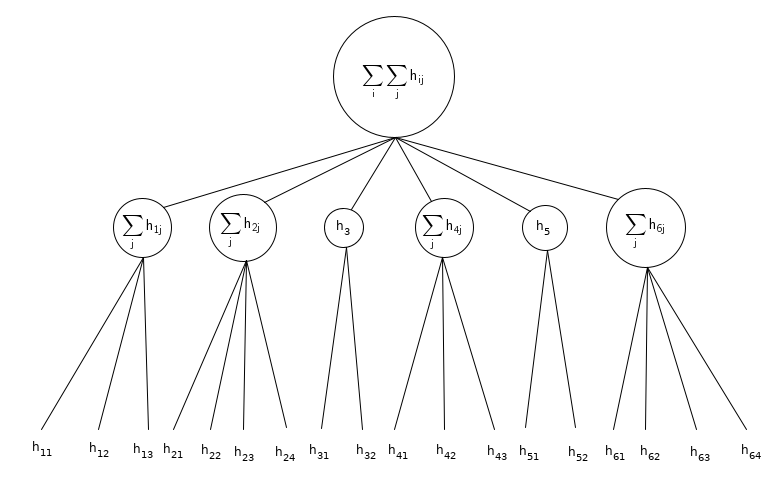
\includegraphics[width=0.7\linewidth]{Screenshot51}
	\caption{Структура временных рядов, необходимых для исследования}
	\label{fig:screenshot51}
\end{figure}


Стоит отметить, что поиск реальных данных, идеально подходящих под такую структуру, затруднен. Обычно для микроэкономических показателей  в первую очередь собираются данные по отдельным компонентам, из которых  можно получить агрегированные ряды, что удовлетворяет свойству аддитивности, однако получить доступ к таким данным сложно. Альтернативой являются макроэкономические данные, при использовании которых стоит учесть, что в общем случае значение верхнего ряда не будет в точности  равно сумме нижних рядов по причине различий в методологиях для рядов разных уровней.
%, используемых для   избежания двойного учета, неточностей и прочих проблем. 

Так например, разбивая ряд ВВП на компоненты по регионам и отраслям, надо учесть, что вообще они будут отражать несколько иной показатель -  валовую добавленную стоимостью (ВДС)~\footnote{Валовая добавленная стоимость определяется как разность между выпуском товаров и услуг и их промежуточным потреблением. ВДС  исчисляется на уровне отраслей и отражает образование первичных доходов в результате процесса производства товаров и услуг.}. Агрегированный ряд, получаемый при суммировании всех ВДС, будет меньше ВВП на величину чистых субсидий на производство и импорт. Такой показатель имеет близкую к единице корреляцию с рядом ВВП, поэтому при точном его прогнозировании мы можем получить представление как об общей динамике всех компонент, составляющих ряд, так и о динамике ряда ВВП.  Так как целью работы является сравнение моделей, для упрощения будем работать с агрегированными показателями по ВВП, являющиеся простой суммой из рядов нижнего уровня. 


Вообще говоря, этот  факт учитывается при расчете вклада компонент, составляющих ряд, в процентное изменение агрегированного показателя, не обладающего свойством аддитивности~\footfullcite{bea3}:  

\begin{equation}\label{key}
 C\% Δ_{i,t} = 100 * \dfrac{q_{i,t}-q_{i,t-1} }{\sum_j q_{j,t-1} } 
\end{equation}

где $q_{i,t}$ - значение $i$-ого ряда в момент времени $t$.
Такой показатель позволяет определить изменения в структуре агрегата, что делает его ценным инструментом экономического анализа.
Если при прогнозировании с помощью иерархических моделей удастся улучшить прогноз агрегированного ряда, то фактически мы также сможем получить достаточно точные прогнозы показателей вклада каждой компоненты.

Для анализа были выбраны три набора данных с описанными выше свойствами, обладающие  разной сезонностью:  квартальные, квартальные сезонно сглаженные и месячные данные. В следующих пунктах будут более подробно   описаны особенности каждого из наборов данных. Ознакомиться с визуальной репрезентацией этих наборов можно в приложении \ref{app-a}.


\subsection{Квартальные данные}

Квартальные данные\footnote{Eurostat: European statistics - Database. URL: \url{https://ec.europa.eu/eurostat/data/database.}} - ряды ВДС по 28 странам Европейского союза (включая Великобританию) в разбивке по основным отраслям\footnote{Eurostat metadata: Annual national accounts (nama10). URL: \url{https://ec.europa.eu/eurostat/cache/
	metadata/en/nama10\_esms.htm}}:

\begin{enumerate}
	\item  'A' - сельское хозяйство, лесное хозяйство и рыболовство;
\item  'B' - промышленность (кроме строительства);
\item  'F' - строительство;
\item  'G'- оптовая и розничная торговля, транспорт, услуги общественного питания и т.д.;
\item  'J'- информация и связь;
\item  'K'- финансовая и страховая деятельность;
\item  'L'- операции с недвижимостью;
\item  'M'- профессиональная, научно-техническая, административная деятельность;
\item  'O'- государственное управление, оборона, образование, здравоохранение и социальная работа;
\item  'R'- искусство, развлечения, отдых и другие виды услуг. 


\end{enumerate}

Данные собраны за период с 2000-Q1 по 2018-Q3. 



%\begin{figure}
%	\centering
%	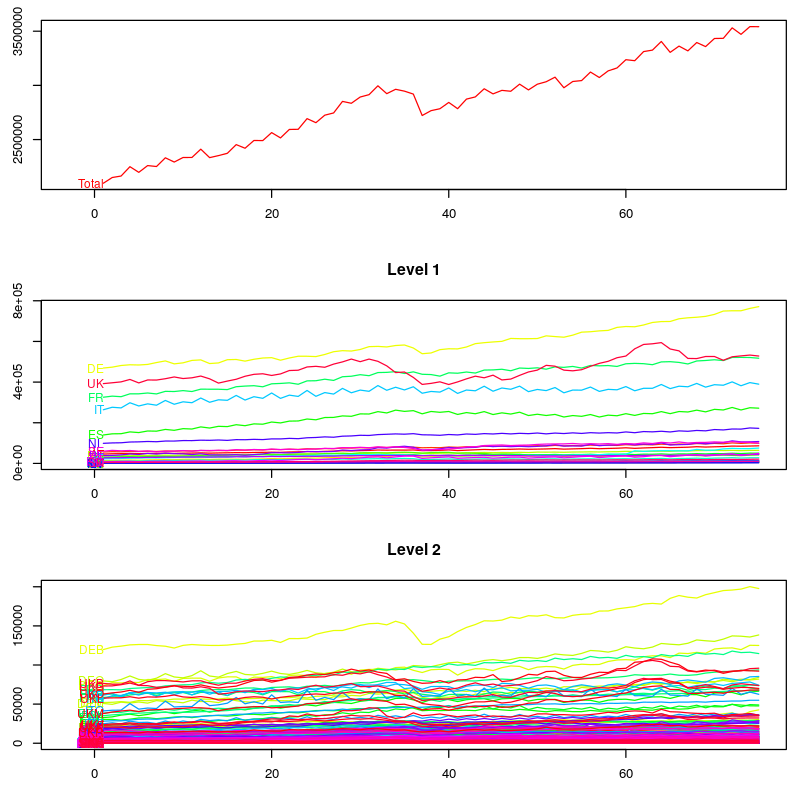
\includegraphics[width=0.7\linewidth]{screenshot001}
%	\caption[Квартальные временные ряды]{Квартальные временные ряды}
%	\label{fig:screenshot001}
%\end{figure}

Разница между совокупным ВВП всех 28 стран, входящих в состав ЕС  и суммой ВДС по всем отраслям для каждого из государств, не превышает  1.5\% от ВВП. 

\subsection{Квартальные сезонно сглаженные данные}

Квартальные сезонно сглаженные данные\footnote{FRED: Economic Data. URL: \url{https://fred.stlouisfed.org/}} - это ряды ВДС  для каждого из 50 штатов Америки с разбивкой на 21 отрасль.  Данные собраны за период с 2005-Q1 по 2018-Q2. 
В этом наборе 11 рядов имели пропуски. По четырем из этих рядов  данные перестали собираться в 2008 году, поэтому эти ряды были исключены целиком. Остальные пропуски  были заполнены \ \ с \ \ помощью экспоненциально взвешенного скользящего среднего \ \  с \ \  шириной \  \  окна 4~\footnote{Алгоритм, используемый в пакете R 'imputeTS'   имеет адаптивный размер окна: в случае длинных промежутков с пропущенными значениями, размер окна постепенно увеличивается до тех пор, пока не появятся как минимум 2 значения не-NA. }. 

Квартальные оценки ВДС в США пересчитываются с учетом сезонных колебаний следующим образом: BEA оценивает соответствующие коэффициенты сезонной корректировки, после чего удаляет из временного ряда среднее влияние изменений, которые обычно происходят примерно в одно и то же время  с одинаковой величиной каждый год. Сезонно несглаженные ряды по этому показателю BEA не публикует.

Показатели по ВДС публикуются в реальном денежном эквиваленте (за базовый год принимается 2012).
Надо отметить, что  значения реальных показателей ВДС по отраслям не обязательно дают в сумме показатель реального ВДС для каждого штата за интересующий период, поскольку относительные цены, используемые в качестве весов для корректировки показателей по отраслям, отличаются от общего уровня цен используемых для корректировки агрегированного показателя. 
Для периодов близких к 2012 году, когда значительных отклонений относительных цен от индекса цен по стране не было, показатель ВДС штата совпадает с суммой ВДС по отраслям, хотя  вообще эта разница не превышает 0.5\% ВВП.
Разница между ВВП США и суммой ВДС по отраслям для каждого штата не превышает 2\%. 


\subsection{Месячные данные}

Месячные данные\footnote{ЕМИСС: государственная статистика: Официальные статистические показатели. URL: \url{https://www.fedstat.ru/}} - показатели рождаемости и смертности по основным причинам  в каждом регионе РФ, дающие в сумме естественный прирост населения помесячно. 
Данные собраны за период с 2006-01 по 2019-01. 


Если для каждого из регионов все показатели из набора данных "Число зарегистрированных умерших по основным классам и отдельным причинам смерти" просуммировать по причинам смерти, значения будут отличаться от показателей  из набора данных "Число зарегистрированных умерших". Такое расхождение объясняется тем, что для перового набора  разрабатываются ряды только по   основным классам и отдельным причинам смерти, имеющим наибольший вес. Также в 2011 году методика разработки показателя была пересмотрена, чтобы соответствовать  Международной статистической классификации\footnote{Демографический ежегодник России: методические пояснения. URL: \url{http://www.gks.ru/bgd/regl/B17\_16/Main.htm}}. 

Для анализа необходимы ряды, в сумме дающие агрегированный ряд естественного прироста населения.  В связи с этим  были выявлены три основные группы причин смертности, причем разница между показателем смертности по каждому региону и суммой по всем причинам смертности была добавлена к ряду "смерть по прочим причинам". В итоге для каждого региона имеем следующее разбиение:   



\begin{enumerate}
	\item 'РО'  -  число рожденных;
	\item  'УБ' - число умерших  из-за болезней (болезней органов дыхания, органов пищеварения, системы кровообращения, инфекционных и паразитарных болезней, новообразований);
\item 'УУ'  -  число умерших по причине убийства и самоубийства;
\item 'УВ'  -  число умерших по прочим причинам (отравление алкоголем, транспортные травмы всех видов и внешние причины).

\end{enumerate}


С 2015 года также собираются данные по республике Крым и городу федерального значения Севастополю. Однако данных нужной сезонности по каждому из классов за 2006-2014 годы Держстат Украины не предоставляет, поэтому ряды по этим регионам были исключены из набора данных. 



%- http://www.ukrcensus.gov.ua Держастат Украины

\section{Выбор моделей прогнозирования рядов нижнего уровня}

Для того чтобы определить, можно ли с помощью комбинирования прогнозов получить более точные прогнозы агрегированных рядов необходимо выбрать модель для прогнозирования нижних рядов. 
Вообще говоря, можно выбирать модели для прогнозирования любого ряда любого уровня независимо друг от друга, оптимизируя, например, метрику качества прогноза. Однако при использовании одной и той же модели, можно  увидеть, есть ли зависимость между выбором параметров модели и методом комбинирования рядов или прогнозов.

%Для сравнение качества прогнозов используется кросс-валидация со скользящим окном. 
Эффективность каждого из методов комбинирования будет проверяться на десяти различных моделях: AR с малым числом лагов (с линейным трендом), AR с линейным и с квадратичным трендом, интегрированная AR, ARMA с линейным трендом, ARIMA, 
ETS с фиксированными параметрами,  ARIMA, ETS и TBATS с автоматическим подбором параметров.~\footnote{Автоматический перебор параметров модели осуществляется с помощью функций R  'auto.arima','ets' и 'tbats' соответственно }



Для выбора параметров в моделях применяется кросс-валидация  со скользящим окном с шагом в одно наблюдение. К рядам нижнего уровня будет применяться модель, для которой среднее по всем подвыборкам RMSE, полученное на кросс-валидации для   агрегированного ряда, будет ниже других в классе используемой модели.  





\begin{table}[H]
	\caption{Параметры моделей }\label{tab11}
	\small\centering\setlength{\extrarowheight}{0.25em}
	\begin{tabular}%{\linewidth}
		{   >{\centering\footnotesize}p{11em} 
			>{\centering\footnotesize}p{8.5em} 
			>{\centering\footnotesize}p{8.5em} 
			>{\centering\footnotesize\arraybackslash}p{8.5em} }\hline
		
		& Квартальные                                  & Сезонно сглаженные               & Месячные                                      \\\hline
AR с линейным трендом (с малым числом лагов) & $(p,d,q)=(2,0,0)$,     

$(P,D,Q)_{4}=(1,0,0)$ & $(p,d,q)=(2,0,0)$                & $(p,d,q)=(2,0,0)$,   

 $(P,D,Q)_{12}=(1,0,0)$  \\
AR с линейным 

трендом                        & $(p,d,q)=(3,0,0)$,   

 $(P,D,Q)_{4}=(2,0,0)$  & $(p,d,q)=(4,0,0)$                & $(p,d,q)=(11,0,0)$, 
   
    $(P,D,Q)_{12}=(2,0,0)$ \\
AR с квадратичным 

трендом                    & $(p,d,q)=(3,0,0)$,   


 $(P,D,Q)_{4}=(2,0,0)$  & $(p,d,q)=(4,0,0)$                & $(p,d,q)=(11,0,0)$,  
 
   $(P,D,Q)_{12}=(2,0,0)$ \\
Интегрированная AR                            & $(p,d,q)=(3,1,0)$,   

 $(P,D,Q)_{4}=(2,1,0)$  & $(p,d,q)=(4,1,0)$                & $(p,d,q)=(4,0,0)$,  
 
   $(P,D,Q)_{12}=(1,1,0)$  \\
ARMA с линейным 

трендом                      & $(p,d,q)=(3,0,1)$, 

   $(P,D,Q)_{4}=(2,0,1)$  & $(p,d,q)=(4,0,1)$                & $(p,d,q)=(4,0,1)$,  
   
     $(P,D,Q)_{12}=(1,0,1)$  \\
ARIMA                                        & $(p,d,q)=(3,1,1)$,  

  $(P,D,Q)_{4}=(2,1,1)$  & $(p,d,q)=(4,1,1)$                & $(p,d,q)=(4,1,1)$, 
  
     $(P,D,Q)_{12}=(1,1,1)$  \\
ARIMA с автоматическим подбором   параметров           & $\lambda = 1$                                & $\lambda = 1$                    & $\lambda = 1$                                 \\
ETS с фиксированными параметрами            & $(E,T,S)=(M,M,M)$ 

$\lambda = 1$            & $(E,T,S)=(A,A,A)$ 

$\lambda = 1$ & $(E,T,S)=(A,Ad,A)$ 

 $\lambda = 1$             \\
ETS с автоматическим подбором     параметров           & $\lambda = 1$                                & $\lambda = 1$                    & $\lambda = 1$                                 \\
TBATS                                        & $\lambda = 1$,  $T=A$                        & $\lambda = 1$,   $T=A$           & $\lambda = 1$,  $T=Ad$                      

	\end{tabular}
\end{table}



		
		Ширина окна для каждого из  набора данных подбиралась в соответствии  длинной ряда и горизонтом прогнозирования в два года таким образом, чтобы при проведении перекрестной проверки с шагом в один год получалось не менее пяти подвыборок. Соответственно для квартальных, сезонно сглаженных и месячных данных имеем:
		\begin{itemize}
			\item для рядов по ВВП ЕС: ширина окна 48 - прогноз на 8 шагов вперед;
			\item для рядов по ВВП США: ширина окна 28 - прогноз на 8 шагов вперед;
			\item для рядов по естественному приросту РФ: ширина окна 84 - прогноз на 24 шага вперед.
		\end{itemize}  
		
		
Различия в ширине окна позволят сравнить модели на относительно небольшой, средней и большой выборке. 
Результат перебора параметров для каждой из основных моделей для всех трех наборов данных представлен в таблице \ref{tab11}. 
		
		
		
		
		


%При прогнозировании на два года вперед, получаем 6 подвыборок для США,  6 подвыборок для ЕС,  5 подвыборок для РФ.  

%один год, для сравнения лучших моделей с шагом в одно наблюдение.
%Для выбора параметров в моделях будем использовать кросс-валидацию с шагом в один год, для сравнения лучших моделей с шагом в одно наблюдение.



%\subsection*{Сравнение качества прогнозов}




Для сравнения качества прогнозов будут использоваться следующие метрики:

\begin{itemize}
	\item  Средняя ошибка (mean error)
\begin{equation}\label{key}
ME = \frac{1}{h} \sum_{i=1}^h(\hat{y}_{t+i|t}-y_{t+i}) 
\end{equation}
\item  Квадратный корень из среднеквадратичной ошибки (root mean square error)
\begin{equation}\label{key}
RMSE = \sqrt{  \frac{1}{h} \sum_{i=1}^h(\hat{y}_{t+i|t}-y_{t+i})^2} 
\end{equation}
\item  Cредняя абсолютная ошибка в процентах  (mean absolute percentage error)
\begin{equation}\label{key}
MAPE = \frac{1}{h} \sum_{i=1}^h \frac{y_{t+i} - \hat{y}_{t+i|t} }{y_{t+i}} * 100\%
\end{equation}

\end{itemize}

Основной метрикой сравнения точности прогнозов моделей будет  RMSE. Средняя ошибка (ME) позволит понять, насколько хорошо модель улавливает тренд в рядах.  MAPE в качестве метрики сравнения точности прогнозов является смещенным показателем, поскольку он будет систематически выбирать модель, прогнозы которой занижены, так как на отрицательные ошибки налагаются большие штрафы, чем на положительные. 
Но зато MAPE позволит сравнивать улучшение качества прогнозов для разных наборов данных, хотя  для набора данных по России MAPE не является показательной метрикой, так как в нем имеются нулевые и близкие к нулю значения.


\section{Группировка рядов третьего уровня по регионам, по типу и по метрике расстояния}

Для данного исследования подбирались наборы данных с трехуровневой структурой, обладающие свойством аддитивности. Это позволяет проверить,  можно ли улучшить прогноз агрегированного ряда используя  комбинации прогнозов каждого из рядов третьего уровня или такое  разбиение рядов на настолько большое число компонент излишне, поскольку приводит к тому, что ошибки прогнозов каждого ряда накапливаются, что ведет  к ухудшению прогноза агрегированного ряда. Если предположить, что разбиение агрегата на компоненты действительно позволяет учесть неоднородность составляющих агрегированного ряда, но оценка большого числа рядов неизбежно приводит к тому, что идиосинкразические    ошибки в сумме растут,     то необходимо найти компромисс между двуми этими эффектами. 

Очевидно, что можно сгруппировать ряды по территориальному признаку (по странам, штатам или регионам) или по типам (для ВВП по отраслям  и для естественного прироста  отдельно ряды по рождаемости и причинам  смерти). Аддитивность  позволяет получить ряды второго уровня просто просуммировав ряды, входящие в одну группу. 

Альтернативным способом  группировки будет кластеризация нормированных  рядов по метрике евклидова расстояния с помощью алгоритма иерархической кластеризации, реализованного в пакете 'dtwclust'.  
Оптимальное число кластеров выбиралось так, чтобы максимизировать значение метрики силуэта. Для всех трех наборов данных оптимальное число кластеров - 25. Визуализацию рядов попавших в один кластер можно увидеть на рисунке~\ref{otkl_14}.

Очевидно, что при использовании процедуры перекрестной проверки необходимо было на каждой итерации получать свою группировку на  кластеры, но для экономии времени проведем кластеризацию на рядах полной длины.


%https://cran.r-project.org/web/packages/dtwclust/vignettes/dtwclust.pdf

%https://cran.r-project.org/web/packages/dtwclust/dtwclust.pdf



\section{Сравнение иерархических моделей}

Для сравнения моделей используется следующая процедура: 

\begin{itemize}
	\item для выполнения перекрестной проверки со скользящим окном с шагом в один год каждый из наборов данных делится на подвыборки: для квартальных данных число подвыборок равно 6, для сезонно сглаженных - 6, для месячных - 5.
	%При прогнозировании на два года вперед, получаем 6 подвыборок для США,  6 подвыборок для ЕС,  5 подвыборок для РФ.  	
	\item модели описанные в таблице \ref{tab11} используются для получения прогноза на 2 года вперед для каждого ряда, каждого уровня для всех трех наборов данных (отдельно с помощью пакета 'hts' оценивается   трехуровневая модель,  отдельно три двухуровневые, сгруппированные по регионам, по классам или по кластерам );
	\item на каждой итерации перекрестной проверки считается RMSFE для агрегированного ряда, RMSFE для невзвешенной суммы всех прогнозов нижнего ряда и RMSFE для скорректированной по OLS суммы всех прогнозов;
	\item для каждого набора данных RMSFE усредняется по  всем подвыборкам и считается процентное изменение  RMSFE для невзвешенной суммы всех прогнозов нижнего ряда и RMSFE для скорректированной по OLS суммы всех прогнозов по сравнению с RMSFE для агрегированного ряда;
	\item полученные значения для трехуровневой и двухуровневых моделей сортируются по  RMSFE   для агрегированного ряда.
\end{itemize}


В результате описанной процедуры получаются таблички, с помощью которых можно наглядно увидеть, как изменился прогноз агрегированного ряда при использовании моделей, учитывающих многоуровневую  структуру данных (Приложение \ref{app-b}). 

Анализируя полученные показатели и визуальное представление анализируемых наборов данных (Приложение \ref{app-a})  можно сделать следующие выводы:

\subsection*{Вывод 1:}

Для невзвешенных прогнозов результаты неоднозначны: для квартальных данных в большинстве случаев при использовании иерархических моделей наблюдается ухудшение  по сравнению прогнозом агрегированного ряда, для сезонно сглаженных рядов для большинства моделей наблюдается улучшение прогнозов, а для месячных на некторых моделях наблюдается улучшение для всех вариантов структуры (трех- и двухуровневой),   на некоторых - ухудшение.
 
	Возможно это объяснется следующими фактами. Для квартальных данных все ряды имеют примерно одинаковую структуру и  ошибки прогнозов не уравновешивают друг друга, а накапливаются.  Для сезонно сглаженных рядов, если посмотреть на метрику  ME, можно заметить, что на всех итерациях перекрестной проверки модель занижает прогнозы, но при прогнозировании отдельных компонент можно с этим бороться, поскольку только малая часть прогнозов рядов приводит к тому что тренд недооценивается, и эти прогнозы выравниваются большим числом прогнозов улавливающих положительный тренд.     Для месячных данных причина неоднозначных результатов заключается в   том, что примерно четверть рядов имеет V-образный тренд (ряды по рождаемости), половина положительный линейный тренд, четверть отрицательный линейный тренд (что видно на рисунке \ref{qwe}   где ряды группируются по типу).  Соответственно для некоторых моделей хорошие  прогнозы  имела большая по размеру группа, а для некоторых меньшая.
	
	
\subsection*{Вывод 2:}

Прогнозы полученные с помощью OLS  корректировки в для квартальных и сезонно сглаженных рядов в большинстве случаев  не отличаются от прогнозов полученных при прогнозировании агрегированного ряда. Доля  прогнозов имеющих распределение отличающееся от распределения прогнозов верхних рядов оказалась небольшой, поэтому оценки для агрегата скорректировались незначительно.   

Для этих наборов данных для невзвешенных  прогнозов наблюдалось  резкое  ухудшение для квартальных и резкое улучшение для сезонно сглаженных рядов, но при корректировке эти резкие изменения сгладились. Учитывая это можно сказать, что при небольшом числе наблюдений, недостаточном для проведения перекрестной проверки модели, стоит    использовать OLS корректировку   прогнозов, которая позволит избежать резких отклонений от настоящих значений, произошедших из-за случайного накопления ошибок, которое может привести, как  к положительному, так и к отрицательному результату.

Стоит заметить, что для месячных данных при OLS корректировке в отличие от     невзвешенной суммы прогнозов наблюдается улучшение прогноза агрегированного ряда практически для любой модели. Исключение составляет только модель с квадратичным трендом. Причина этому заключается в том, что только четверть рядов имеют V-образную форму, такую же, как у  агрегированного  ряда.  Поэтому корректировка прогнозов агрегированного ряда на априори худшие  прогнозы, имеющие сильно отличающееся распределение приводит к тому, что прогнозы сильно корректируются в сторону ухудшения. 

По той же причине для AR модели с большим числом лагов с линейным трендом для модели с трехуровневой структурой наблюдается ухудшение, поскольку треть рядов прогнозируется по подходящей модели, а четверть по распределению  совпадает   с некачественным агрегированным прогнозом.  

\subsection*{Вывод 3:}

Если сравнивать эффективность использования различных видов группировки можно сказать, что  в среднем ее использование  перед получением прогнозов отдельных рядов приносит положительный результат. Причем для квартальных данных лучше всего работает группировка по отраслям (как со взвешиванием, так и без), для сезонно сглаженных для обоих способов лучше заметное улучшение наблюдается при группировке по кластерам, а для месячных данных для невзвешенных прогнозов более эффективна группировка по кластерам, а для взвешенных - группировка по типам.


Во всех случаях группировка по территориальному признаку оказывалась чуть хуже других типов группировок, но по отношению к трехуровневой модели без группировки улучшение происходило не во всех случаях.  

Вообще говоря, OLS корректировка происходила с учетом второго уровня собираемого именно по территориальному признаку, поэтому имело бы смысл проводить OLS корректировку по  рядам третьего уровня с более подходящей  для каждого из наборов данных группировкой второго уровня. 


Возможная причина таких результатов заключается в том, что при группировке по территориальному признаку ряды приобретают 
некую обособленность друг от друга, которая в половине случаев позволяет улучшить прогнозы по сравнению с агрегированным рядов, поскольку используется дополнительная информация о ряде, а в половине добавляет непрогнозируемую ошибку, которая накапливается при суммировании. 

При анализе рисунка \ref{qwe} группировка по типу приводит к тому, что в большинстве случаев ряды с общей тенденцией попадают в относительно небольшое число классов, причем ряды похожи друг на друга не только статистически, но и экономический смысл у ни один, а соответственно и реакция их на внешние непрогнозируемые шоки с большей вероятностью будет похожей. 

Группировка по кластерам в общем-то приносит положительные результаты, однако нельзя забывать, что на определенный момент времени ряды могли случайно попасть в один кластер. Поскольку согласно выбранной метрике кластеризации учитывалась только близость нормированных рядов без учета каких-либо экономических факторов. По этой причине то что  в некоторых случаях  прогнозы полученные после группировки по кластерам оказывалась хуже других, можно объяснить  тем, что  алгоритм  уловил зависимости, которых на самом деле нет.  



%\begin{table}[ht]
%	\centering
%	\begin{tabular}{rrrrr}
%		\hline
%		& ME & RMSE & MAPE & MASE \\ 
%		\hline
%		RW with drift  & 0.02 & 34.78 & 0.82 & 0.29 \\ 
%		Auto ARIMA & 70.50 & 71.55 & 2.03 & 0.73 \\ 
%		ARIMA & 72.67 & 73.73 & 2.09 & 0.75 \\ 
%		RW & 77.53 & 100.92 & 2.52 & 0.91 \\ 
%		ETS & 100.50 & 108.39 & 2.87 & 1.04 \\ 
%		Theta & 103.38 & 109.50 & 2.96 & 1.07 \\ 
%		SNaive & 134.86 & 146.04 & 3.86 & 1.40 \\ 
%		\hline
%	\end{tabular}
%\end{table}
%
%\begin{tabular}{rrrrr}
%	\hline
%	& ME & RMSE & MAPE & MASE \\ 
%	\hline
%	RW with drift  & 0.02 & 34.78 & 0.82 & 0.29 \\ 
%	Auto ARIMA & 70.50 & 71.55 & 2.03 & 0.73 \\ 
%	ARIMA & 72.67 & 73.73 & 2.09 & 0.75 \\ 
%	RW & 77.53 & 100.92 & 2.52 & 0.91 \\ 
%	ETS & 100.50 & 108.39 & 2.87 & 1.04 \\ 
%	Theta & 103.38 & 109.50 & 2.96 & 1.07 \\ 
%	SNaive & 134.86 & 146.04 & 3.86 & 1.40 \\ 
%	\hline
%\end{tabular}
%



\chapter*{Заключение}
\addcontentsline{toc}{chapter}{Заключение}



В этом исследовании продемонстрированы различные подходы к прогнозированию временных рядов с многоуровневой иерархической структурой, позволяющие учитывать взаимозависимости как между самими рядами, так и между  прогнозами.  Эффективность этих методов проверялась на трех различных наборов данных, длина рядов в которых позволяла проводить перекрестную проверку.

В результате проведенного анализа были получены три основных вывода:  эффективность  моделей прогнозирования  агрегированных рядов с помощью моделей, учитывающих многоуровневую структуру данных,  сильно варьируется для разных наборов данных и зависит от структуры рядов-компонент   по отдельности;
комбинирование прогнозов с помощью OLS-корректировки позволяет устранить случайное  отклонение невзвешенной суммы прогнозов от прогноза агрегированного ряда из-за накопления идиосинкразических ошибок;
предварительная группировка с целью снижения вероятности накопления ошибок  рядов нижнего уровня приносит положительный результат. 


Отметим, что результат применения какого-либо метода сильно зависит от характеристик  данных, их свойств и структуры. Целью этого исследования было улучшить прогнозы агрегированного ряда. Однако проведенное исследование показало, что использование иерархических моделей может помочь при  анализе сложной структуры специфических наборов данных.

%Взвешивание прогнозов повышает точность прогнозов, по сравнению с невзвешенной суммой прогнозов рядов третьего уровня

%Прогнозирование рядов второго уровня дает сопоставимые прогнозы с прогнозом агрегированного ряда, если спецификация модели ряда первого уровня совпадает со спецификацией его компонент. 






% теоретическую и практическую значимость работы (если работа претендует на значи-мые результаты в этих аспектах)

%Практическая значимость работы заключается в том, что при анализе результатов применения изучаемых методов на трех наборах данных (с разной сезонностью, числом наблюдений и рядов на каждом уровне)   с использованием перекрестной проверки (кросс-валидации) можно протестировать методы на независимых данных, а следовательно получить более устойчивые  выводы. 





\newpage

\nocite{*}  %Чтобы в список литературы напечаталичь все источники из bib-файла

% Если нам хочется, чтобы в списке литературы были не полуторные интервалы можно воспользоваться следующим приёмом: 
\begingroup
\setstretch{1}
\printbibliography[title = Список литературы]
\addcontentsline{toc}{chapter}{Список литературы}

\endgroup







%%%%%%%%%%%%%%%%%%%% Приложения %%%%%%%%%%%%%%%%%%%%

\appendix
\renewcommand{\thechapter}{\Asbuk{chapter}}

%%%%%%%%%% titlesec для приложений
\titleformat{\chapter}
 {\normalfont\bfseries\large}{\chaptertitlename~\thechapter}{0.25em}{\normalfont}


\titlecontents{chapter}
              [0 em] % 
              {\normalsize}
              {\makebox[7em][l]{Приложение \thecontentslabel}}
              {Приложение }
              {\titlerule*[10pt]{.}\contentspage}


\chapter[Визуализация временных рядов с трехуровневой структурой]{Визуализация временных рядов с трехуровневой структурой}\label{app-a}
\begin{figure}[H]
	\caption{Временные ряды полученные путем агрегирования рядов третьего уровня }
	\label{otkl_1}

	\centering\footnotesize{Квартальные данные - ВВП ЕС }
		
	\begin{minipage}[H]{0.4\linewidth}
		\centering{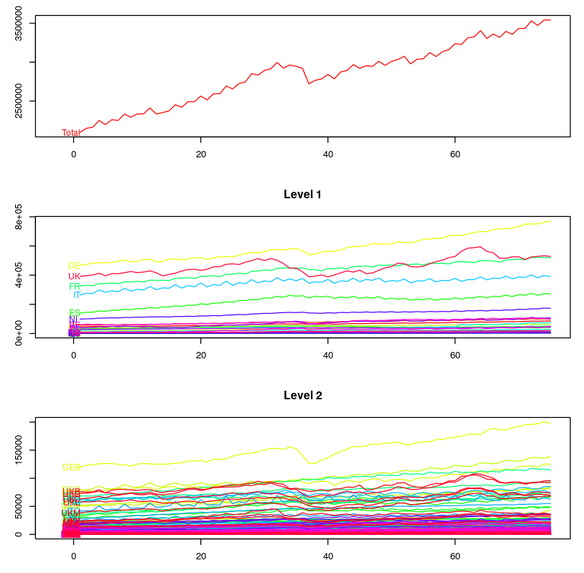
\includegraphics[width=1\linewidth]{screenshot002}}
	\end{minipage}
	\begin{minipage}[H]{0.4\linewidth}
		\centering{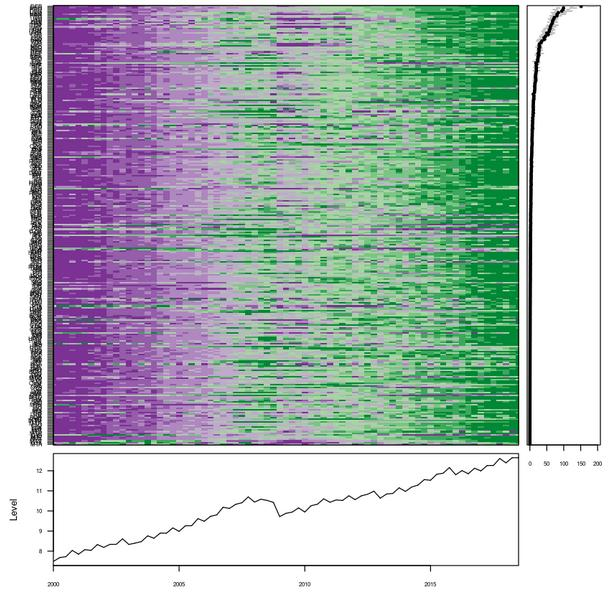
\includegraphics[width=1\linewidth]{screenshot005}}
	\end{minipage}


	\centering\footnotesize{Сезонно сглаженные данные - ВВП США}
	
	\begin{minipage}[H]{0.4\linewidth}
		\centering{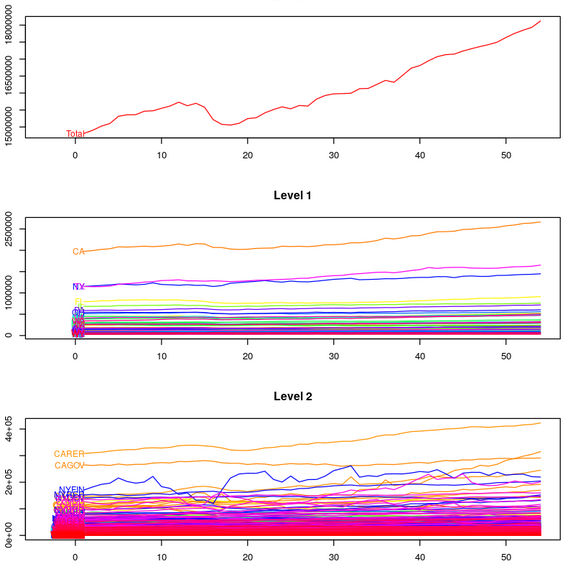
\includegraphics[width=1\linewidth]{screenshot003}}
	\end{minipage}
\begin{minipage}[H]{0.4\linewidth}
	\centering{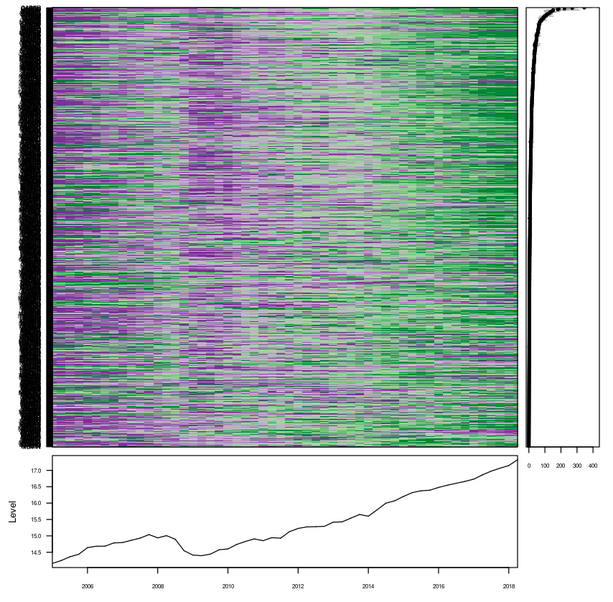
\includegraphics[width=1\linewidth]{screenshot006}}
\end{minipage}


	\centering\footnotesize{Месячные данные - естественный прирост РФ  }
	
	\begin{minipage}[H]{0.4\linewidth}
		\centering{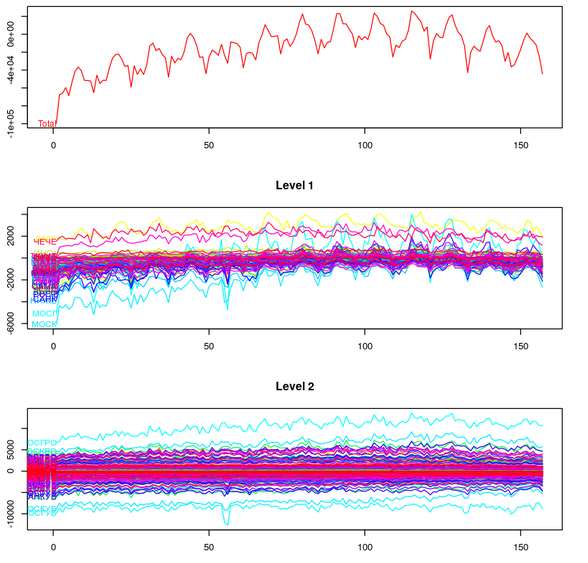
\includegraphics[width=1\linewidth]{screenshot004}}
	\end{minipage}
%	\hfill
\begin{minipage}[H]{0.4\linewidth}
	\centering{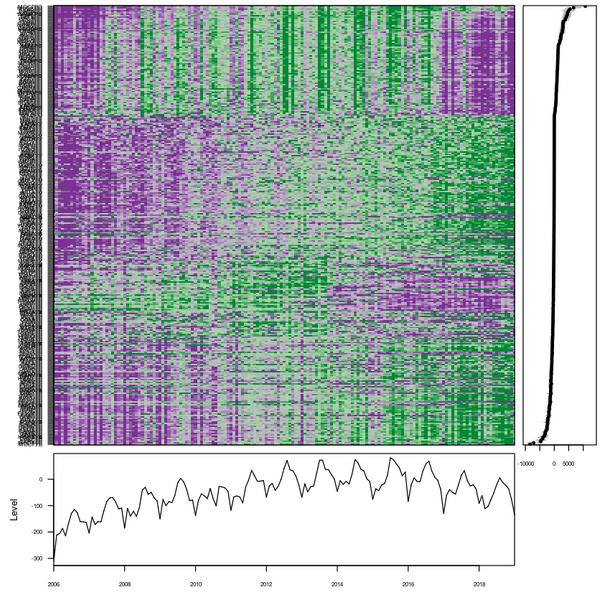
\includegraphics[width=1\linewidth]{screenshot007}}
\end{minipage}
\end{figure}
\newpage



\begin{figure}[H]
	\caption{Временные ряды сгруппированные по территориальному признаку и  по типу }
	\label{qwe}
	
	\centering\footnotesize{Квартальные данные - ВВП ЕС  }
	
	\begin{minipage}[H]{0.4\linewidth}
		\centering{\footnotesize{по 28 странам  }
			\\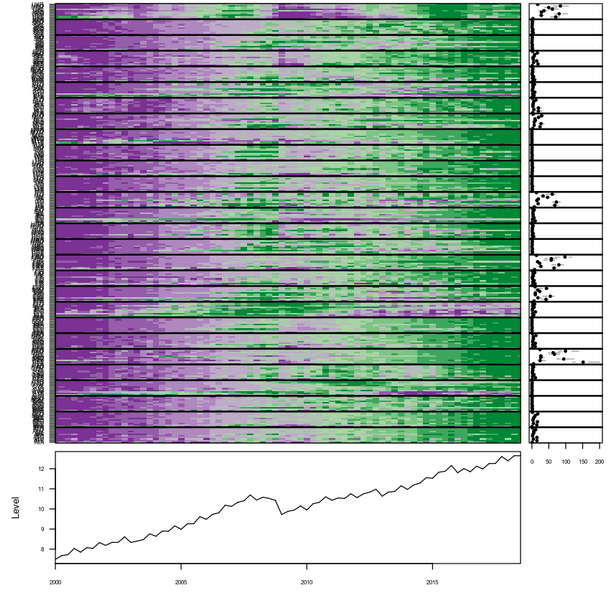
\includegraphics[width=1\linewidth]{screenshot008}}
	\end{minipage}
	\begin{minipage}[H]{0.4\linewidth}
		\centering{\footnotesize{по 10 отраслям  }
			\\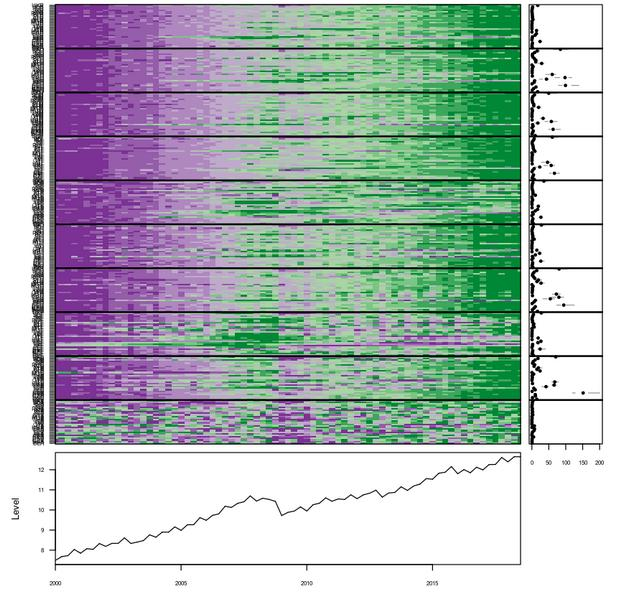
\includegraphics[width=1\linewidth]{screenshot009}}
	\end{minipage}
	
	
	\centering\footnotesize{Сезонно сглаженные данные - ВВП США}
	
	\begin{minipage}[H]{0.4\linewidth}
		\centering{\footnotesize{по 50 штатам  }
			\\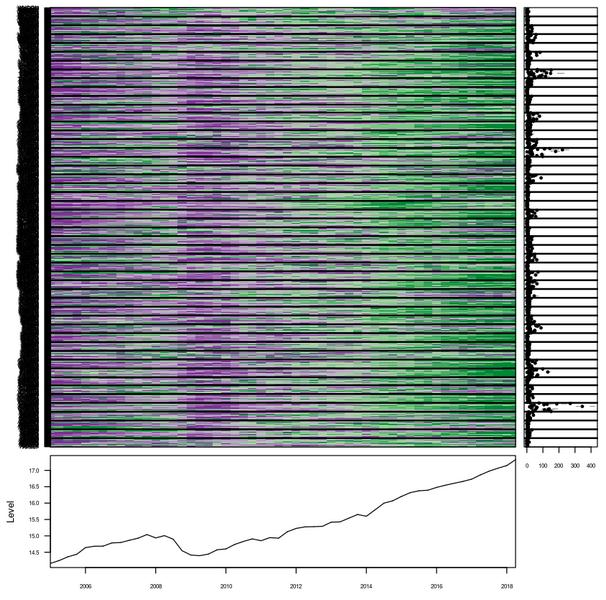
\includegraphics[width=1\linewidth]{screenshot010}}
	\end{minipage}
	\begin{minipage}[H]{0.4\linewidth}
		\centering{\footnotesize{по 21 отрасли   }
			\\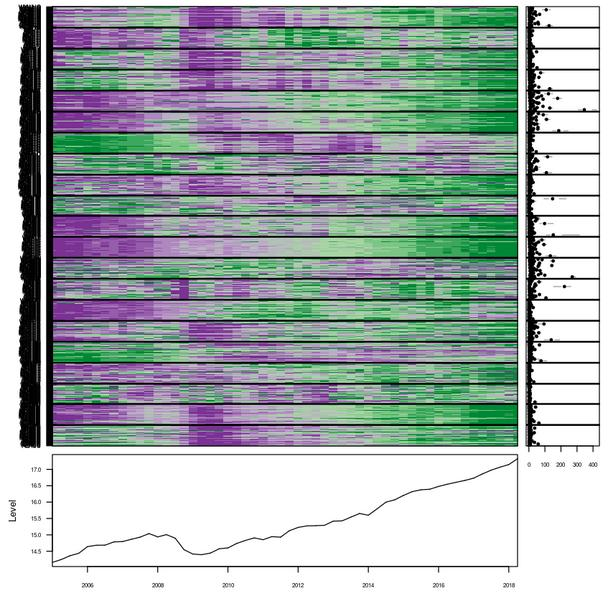
\includegraphics[width=1\linewidth]{screenshot011}}
	\end{minipage}
	
	
	\centering\footnotesize{Месячные данные - естественный прирост РФ  }
	
	\begin{minipage}[H]{0.4\linewidth}
		\centering{\footnotesize{по 80 регионам }
			\\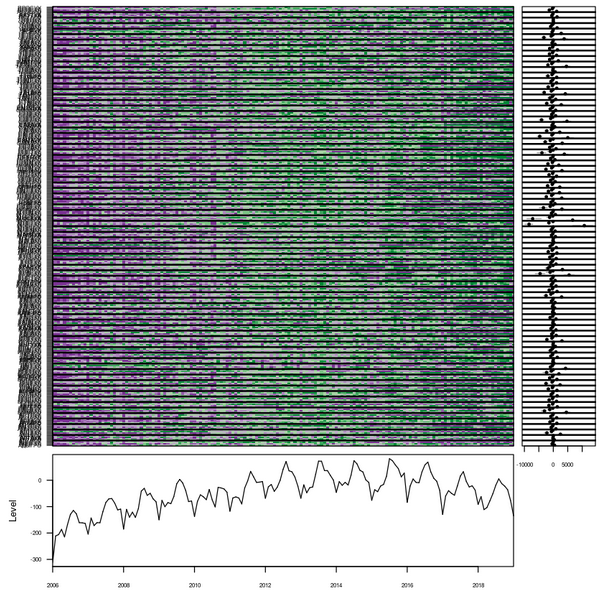
\includegraphics[width=1\linewidth]{screenshot012}}
	\end{minipage}
	%	\hfill
	\begin{minipage}[H]{0.4\linewidth}
		\centering{\footnotesize{по 4 классам   }
			\\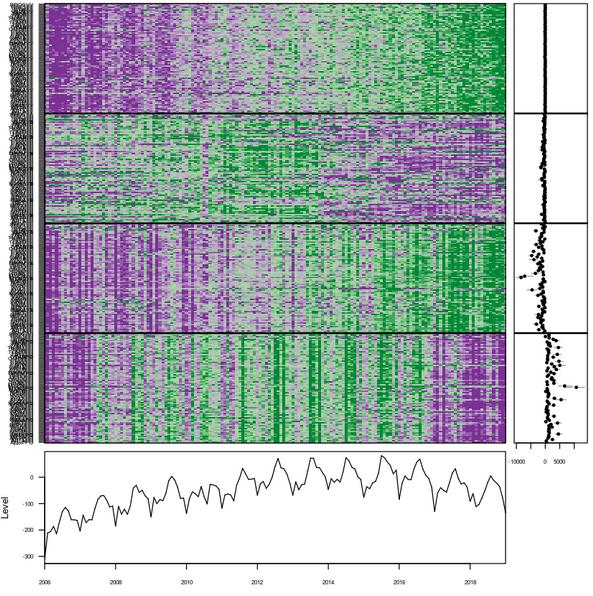
\includegraphics[width=1\linewidth]{screenshot013}}
	\end{minipage}
\end{figure}
\newpage



\begin{figure}[H]
	\caption{Временные ряды сгруппированные по метрике расстояния}
	\label{otkl_14}
	
	\centering\footnotesize{Квартальные данные - ВВП ЕС  }
	
	\begin{minipage}[H]{0.4\linewidth}
		\centering{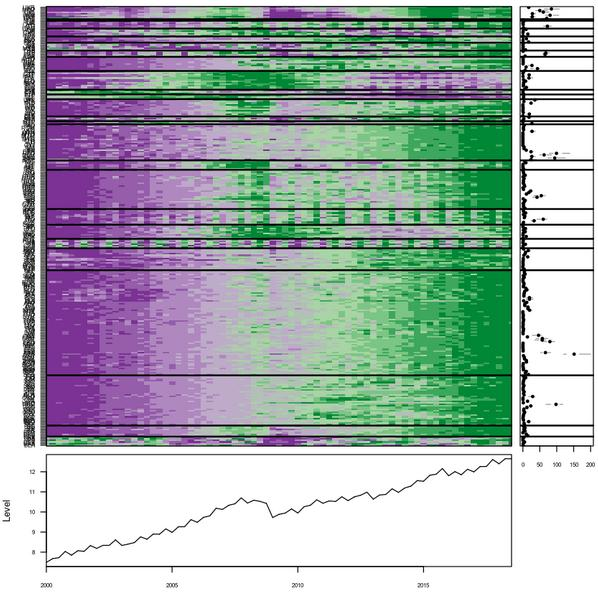
\includegraphics[width=1\linewidth]{screenshot014}}
	\end{minipage}
%	\begin{minipage}[H]{0.4\linewidth}
%		\centering{\footnotesize{по 10 отраслям  }
%			\\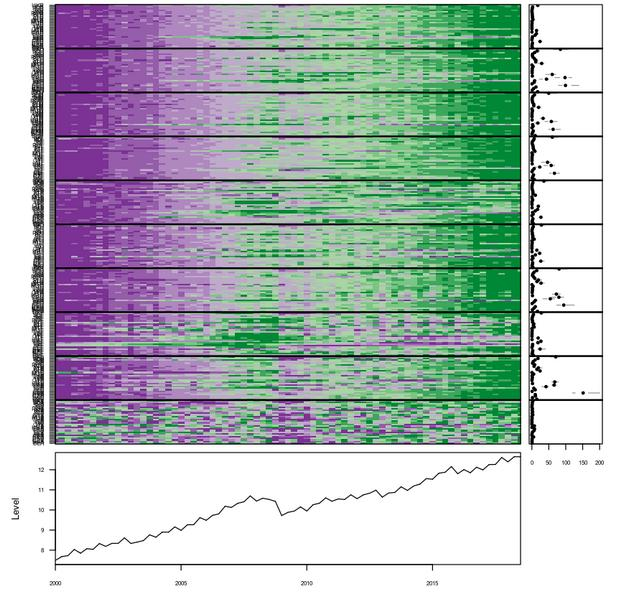
\includegraphics[width=1\linewidth]{screenshot009}}
%	\end{minipage}
	
	
	\centering\footnotesize{Сезонно сглаженные данные - ВВП США}
	
	\begin{minipage}[H]{0.4\linewidth}
	\centering{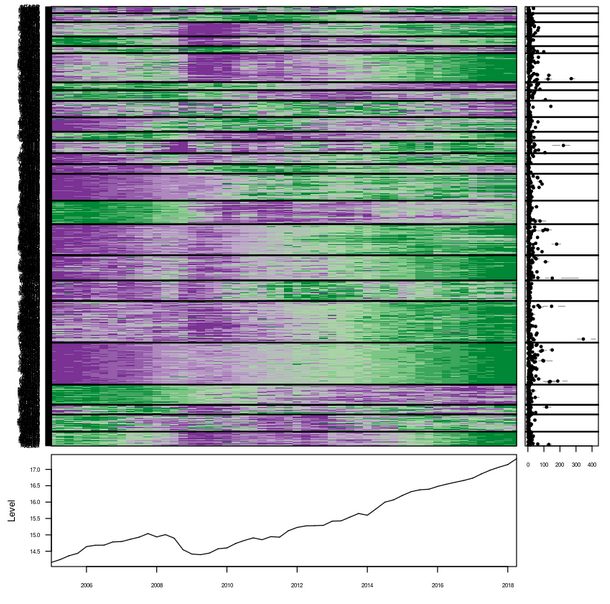
\includegraphics[width=1\linewidth]{screenshot015}}
\end{minipage}
%	\begin{minipage}[H]{0.4\linewidth}
%		\centering{\footnotesize{по 21 отрасли   }
%			\\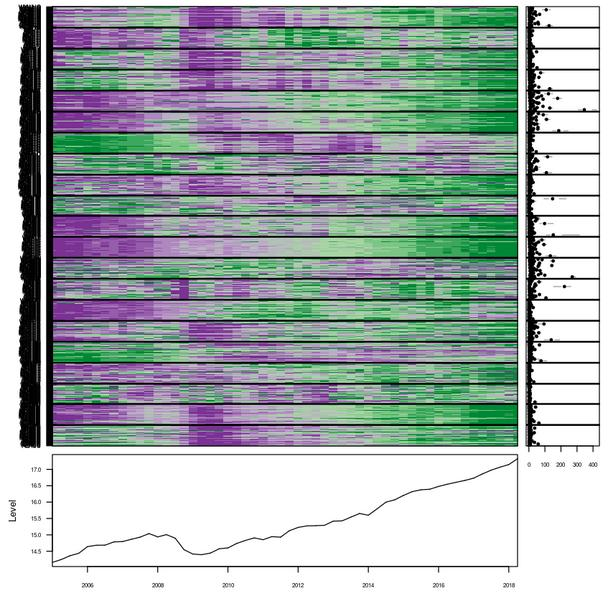
\includegraphics[width=1\linewidth]{screenshot011}}
%	\end{minipage}
	
	
	\centering\footnotesize{Месячные данные - естественный прирост РФ  }
	
	\begin{minipage}[H]{0.4\linewidth}
	\centering{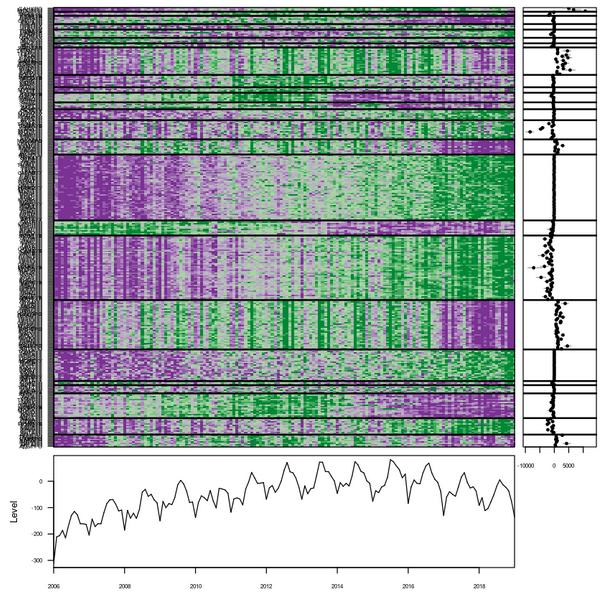
\includegraphics[width=1\linewidth]{screenshot016}}
\end{minipage}
	%	\hfill
%	\begin{minipage}[H]{0.4\linewidth}
%		\centering{\footnotesize{по 4 классам   }
%			\\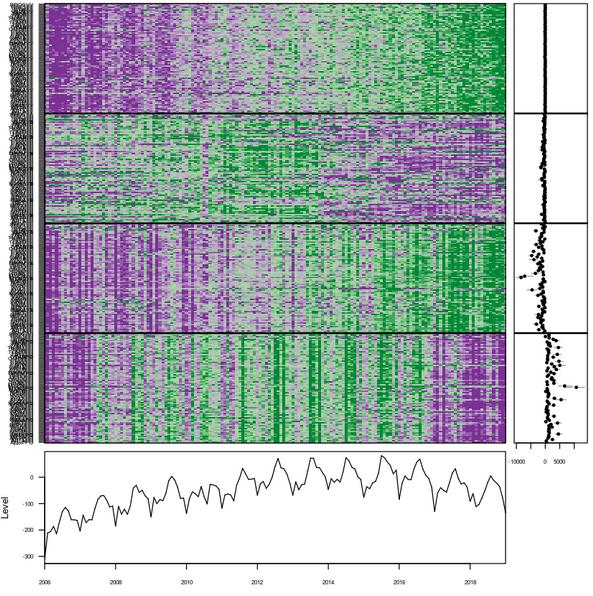
\includegraphics[width=1\linewidth]{screenshot013}}
%	\end{minipage}
\end{figure}
\newpage



\chapter[Сравнение иерархических моделей]{Сравнение иерархических моделей}\label{app-b}


\begin{figure}[H]
%	\caption{Временные ряды сгруппированные по территориальному признаку и  по типу }
	\label{otkl_1}
	
	\centering\footnotesize{Квартальные данные - ВВП ЕС  }
	
	\begin{minipage}[H]{0.4\linewidth}
		\centering{\footnotesize{невзвешенные прогнозы}
			\\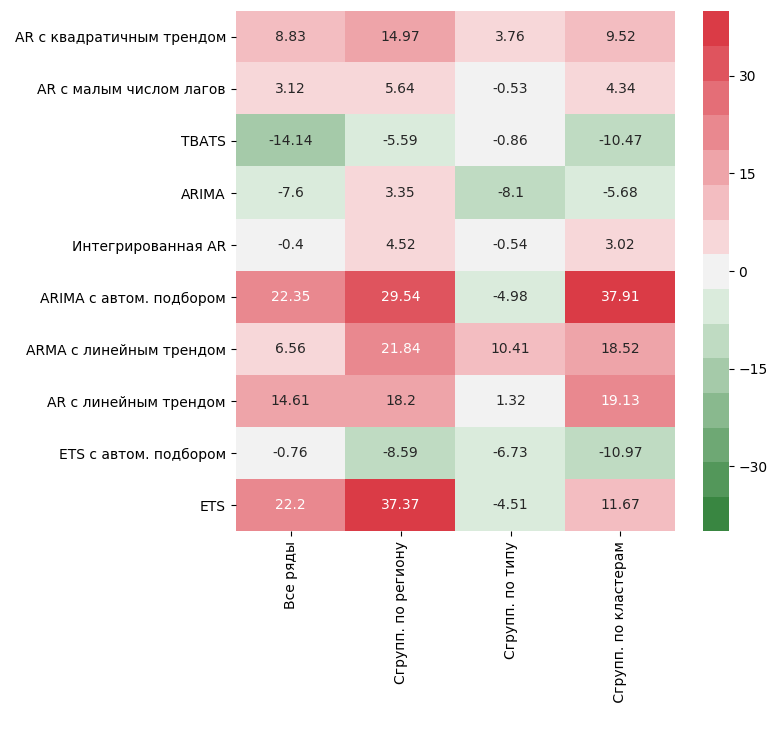
\includegraphics[width=1\linewidth]{screenshot020}}
	\end{minipage}
		\hfill
	\begin{minipage}[H]{0.4\linewidth}
		\centering{\footnotesize{ OLS взвешенные прогнозы }
			\\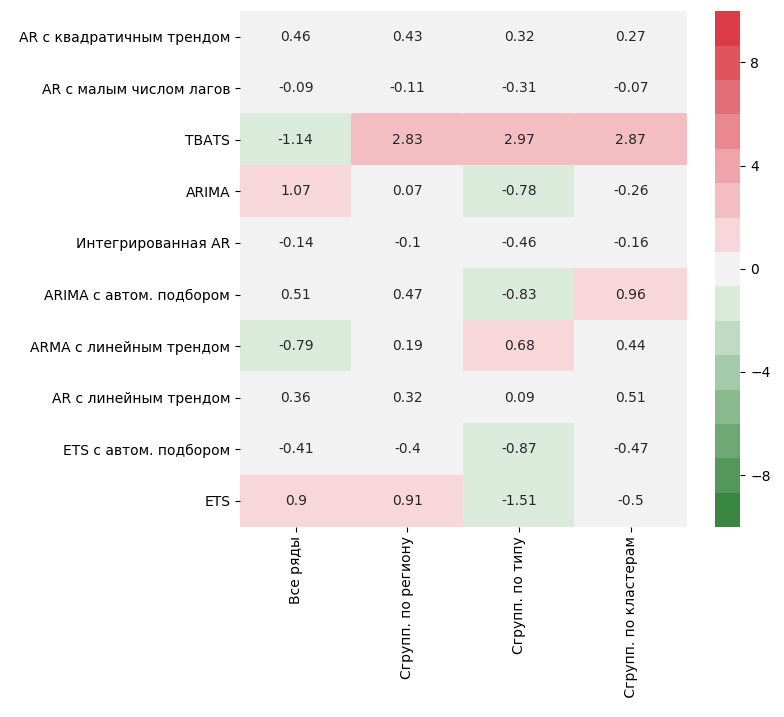
\includegraphics[width=1\linewidth]{screenshot017}}
	\end{minipage}
	
	
	\centering\footnotesize{Сезонно сглаженные данные - ВВП США}
	
	\begin{minipage}[H]{0.4\linewidth}
		\centering{\footnotesize{невзвешенные прогнозы  }
			\\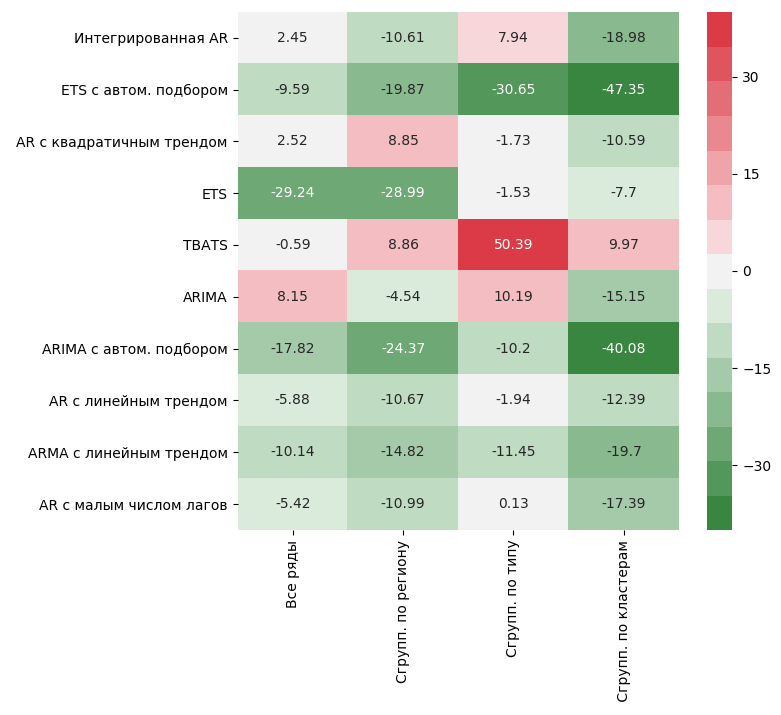
\includegraphics[width=1\linewidth]{screenshot021}}
	\end{minipage}
		\hfill
	\begin{minipage}[H]{0.4\linewidth}
		\centering{\footnotesize{OLS взвешенные прогнозы  }
			\\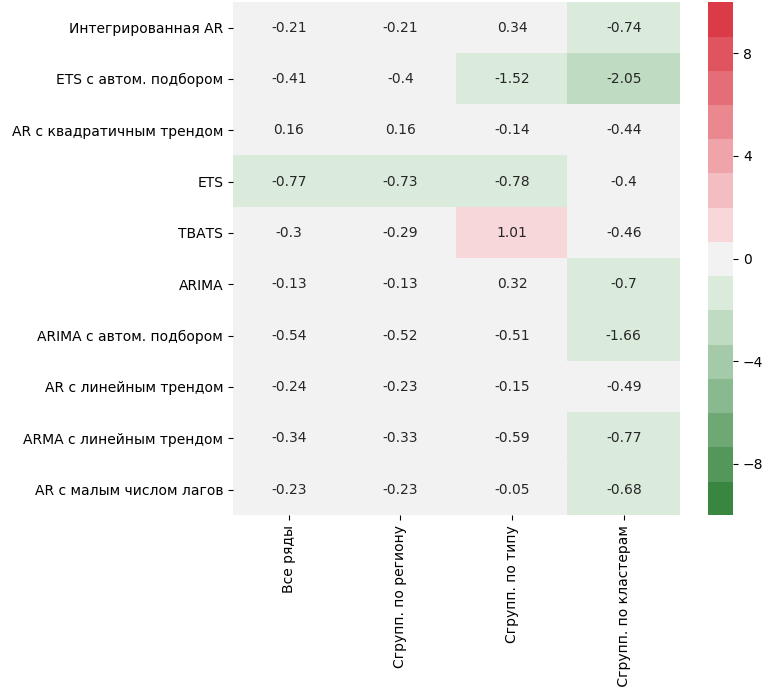
\includegraphics[width=1\linewidth]{screenshot018}}
	\end{minipage}
	
	
	\centering\footnotesize{Месячные данные - естественный прирост РФ  }
	
	\begin{minipage}[H]{0.4\linewidth}
		\centering{\footnotesize{невзвешенные прогнозы }
			\\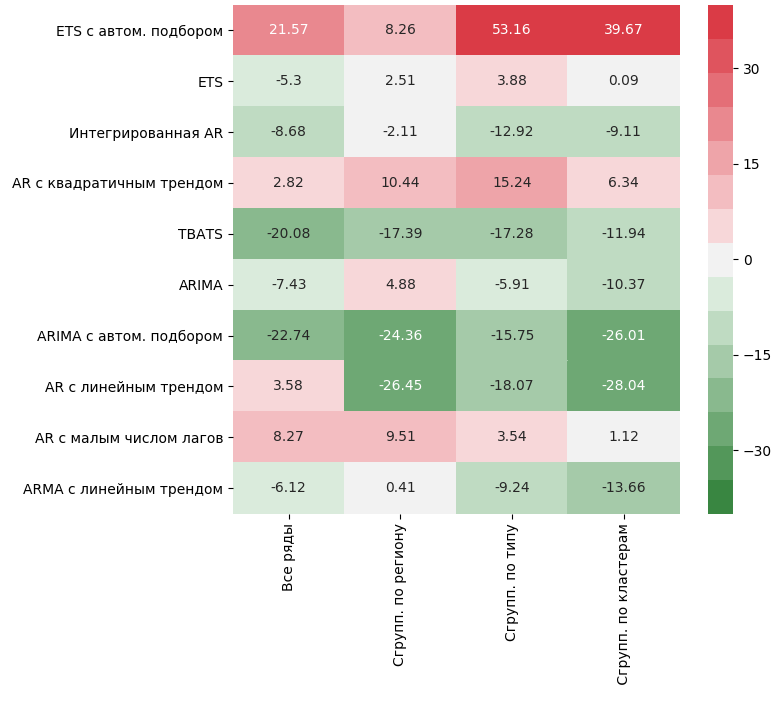
\includegraphics[width=1\linewidth]{screenshot022}}
	\end{minipage}
		\hfill
	\begin{minipage}[H]{0.4\linewidth}
		\centering{\footnotesize{OLS взвешенные прогнозы }
			\\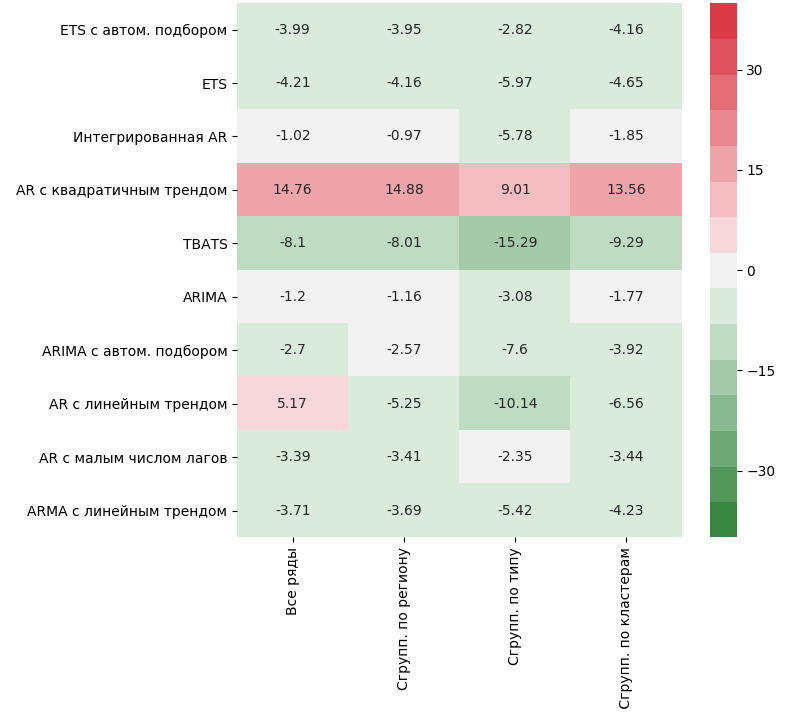
\includegraphics[width=1\linewidth]{screenshot019}}
	\end{minipage}
\end{figure}
\newpage




\thispagestyle{empty}

Выпускная квалификационная работа выполнена мной совершенно самостоятельно. Все использованные в работе материалы и концепции из опубликованной научной литературы и других источников имеют ссылки на них.

\vspace{2ex}

 Объем работы  \rule{2em}{0.5pt} листа(ов).

\vspace{2ex}

 Объем приложений \rule{2em}{0.5pt} листа(ов).

\vspace{4ex}

\noindent << \rule{1em}{0.5pt} >> \rule{5em}{0.5pt} 20 \rule{1.4em}{0.5pt} г. 

\vspace{4ex}



\noindent \rule{11em}{0.5pt} 
\hspace{8em} / Касьянова Ксения Алексеевна /

\hspace{5ex} \footnotesize (подпись)


%\hfill\makebox[6em]{\hfill\footnotesize (подпись) \hfill }


\end{document}
